\documentclass[11pt]{article}

\usepackage[margin=1in]{geometry}
\usepackage{amsmath, amssymb}
\usepackage{listings}
\usepackage{xcolor}
\usepackage{hyperref}
\usepackage{enumitem}
\usepackage{titlesec}
\usepackage{parskip}
\usepackage{booktabs}
\usepackage{tcolorbox}
\usepackage{tikz}
\usetikzlibrary{arrows.meta, positioning, shapes.geometric, shapes.misc}

\lstset{
    basicstyle=\ttfamily\small,
    keywordstyle=\color{blue}\bfseries,
    commentstyle=\color{gray}\itshape,
    stringstyle=\color{red},
    frame=single,
    breaklines=true,
    showstringspaces=false,
    tabsize=4
}

\newtcolorbox{keyidea}[1][]{colback=blue!5, colframe=blue!50!black,
    fonttitle=\bfseries, title=Key Idea, #1}

\newtcolorbox{keytip}[1][]{colback=green!5, colframe=green!50!black,
    fonttitle=\bfseries, title=Tip, #1}

\newtcolorbox{keyintuition}[1][]{colback=orange!5, colframe=orange!50!black,
    fonttitle=\bfseries, title=Intuition, #1}

\title{\textbf{CS3210: Operating Systems} \\ Lecture 7 --- Copy-on-Write Fork}
\author{John Kim \\ Georgia Institute of Technology}
\date{February 5, 2026}

\begin{document}
\maketitle
\tableofcontents
\newpage

% ============================================================
\section{Introduction: The Lazy Design Principle}
% ============================================================

Virtual memory provides far more than a mechanism to translate virtual addresses to physical ones. The \textbf{page table} and the underlying paging hardware infrastructure introduce a layer of indirection that allows the operating system to interpose on every memory access and fundamentally change how the machine behaves. Rather than directly exposing physical memory to applications, the OS can observe, monitor, change, and redirect memory operations through sophisticated page table manipulation.

The core insight driving virtual memory optimization is simple: \emph{we get to lie and be lazy}. The OS need not immediately satisfy requests or fulfill commitments; instead, it can defer action until forced to act by the application. This lazy design principle underpins nearly all advanced virtual memory techniques. When a process calls \texttt{fork()}, for example, the OS could immediately duplicate all physical memory pages belonging to the parent. But this is wasteful. Instead, the OS can lie to both the parent and child, claiming they each have their own private memory while physically sharing the same pages. The child will not modify most of that memory immediately; many pages will never be written at all. So why copy?

This lecture focuses on the first and most elegant VM trick enabled by paging: \textbf{copy-on-write (CoW) fork}. We explore how the OS exploits page permissions and page faults to defer copying until the moment a child process actually attempts to modify a page.

% ============================================================
\section{Virtual Memory Tricks: The Toolbox}
% ============================================================

Paging enables a rich set of powerful optimizations and features. The following list outlines the major VM tricks that modern operating systems employ:

\begin{enumerate}
    \item \textbf{Copy-on-write fork} --- defer physical page copying until child writes.
    \item \textbf{Demand paging / lazy allocation} --- allocate and zero-fill pages on first access, not at process creation.
    \item \textbf{On-demand zero-filled pages} --- maintain a single zero page and copy-on-write when needed.
    \item \textbf{Virtual allocation} --- allow applications to reserve address space without committing physical memory.
    \item \textbf{Virtual shared memory} --- allow multiple processes to share the same physical pages.
    \item \textbf{Memory-mapped files} --- map file contents into the address space.
    \item \textbf{Paging to disk} --- swap infrequently used pages to secondary storage.
    \item \textbf{Memory oversubscription} --- run more memory-demanding workloads than physical RAM permits.
\end{enumerate}

All of these rely on the same underlying mechanism: the page table as a tool for OS interposition. This lecture explores copy-on-write fork in detail. The principles and engineering challenges that arise are representative of the broader class of VM tricks.

% ============================================================
\section{Copy-on-Write Fork: The Problem Statement}
% ============================================================

To understand the motivation for copy-on-write fork, consider the naive approach that many early operating systems used. When \texttt{fork()} is called, the OS must create a new process with an independent virtual address space. The straightforward implementation is to \emph{duplicate everything}: copy all physical pages mapped in the parent's address space into new physical frames, and construct new page tables for the child that point to these copied pages.

Suppose the parent process has allocated three 4-KB pages with contents \texttt{0xcafe}, \texttt{0xbeef}, and \texttt{0x0507}. The parent's page directory points to page table pages, which in turn point to these three physical pages. Under naive fork, the OS would:

\begin{enumerate}
    \item Allocate three new physical frames.
    \item Copy the contents from the parent's three pages into these new frames.
    \item Construct a new page directory and page table hierarchy for the child.
    \item Point the child's page tables to the newly copied frames.
\end{enumerate}

The result is complete physical duplication: now six 4-KB frames are in use, one set for each process. The operation is \textbf{O(n)} in the number of mapped pages, which can be hundreds of megabytes or even gigabytes in a real system.

\begin{keyidea}
The fundamental waste in naive fork is that most forked children will never write to most pages. In fact, \texttt{fork()} is almost always immediately followed by \texttt{exec()}, which overwrites the entire address space. Copying the entire virtual address space is pessimistic and expensive.
\end{keyidea}

This inefficiency motivated the design of copy-on-write fork, which asks a different question: \emph{what if we do not copy immediately?}

% ============================================================
\section{Preserving State Efficiently with Copy-on-Write}
% ============================================================

The key insight of copy-on-write fork is to defer physical page duplication. When \texttt{fork()} is called, both the parent and child processes initially \textbf{share the same physical pages}. The child's page table entries point to the exact same physical frames as the parent's page table entries.

In the example above, instead of allocating six pages, only three physical frames are needed. Both parent and child hold page table entries that reference the same three frames: the frame containing \texttt{0xcafe}, the frame containing \texttt{0xbeef}, and the frame containing \texttt{0x0507}. The child's page directory and page table structure are distinct (so each process has its own page tables), but the pages themselves are shared.

This sharing is not a violation of process isolation; it is safe because we use a clever trick: we make the shared pages \textbf{read-only}. The \texttt{W} (Writable) bit in the page table entry is cleared for both parent and child. If either process attempts to \emph{read} the page, the access succeeds silently. If either process attempts to \emph{write} to the page, the CPU raises a page fault because the \texttt{W} bit is unset.

When a page fault occurs, the OS page fault handler checks whether the fault was due to a write to a read-only copy-on-write page. If so, it:

\begin{enumerate}
    \item Allocates a new physical frame.
    \item Copies the contents of the shared page into this new frame.
    \item Updates the faulting process's page table entry to point to the new frame and sets the \texttt{W} bit.
    \item Returns from the page fault handler; the write now proceeds.
\end{enumerate}

The child process has its copy, the parent retains the original. After this copy, each process has exclusive access to its copy and can write to it freely. Meanwhile, pages that were never written by either process remain shared indefinitely, amortizing the cost of the fork operation across the set of pages that are actually modified.

\begin{keyintuition}
Copy-on-write is a beautiful example of lazy evaluation in systems design. The OS recognizes that the common case is that most pages are never written after fork, so it optimistically shares pages and only pays the cost of copying on writes, which are typically rare. This is \emph{optimistic} rather than \emph{pessimistic}. The opposite would be to eagerly copy all pages on fork and only share later if neither process writes---which is precisely backwards.
\end{keyintuition}

% ============================================================
\section{Shared Page Table Pages: Aggressive Deduplication}
% ============================================================

We can push the optimization even further. If we are willing to share physical pages, why not also share page table pages themselves? Under this more aggressive scheme, two processes can share not only the physical pages they read from but also the intermediate page table structures.

In the example above, Process 1 and Process 2 could both point to the same Page Directory (PD1). This PD1 could point to shared page table pages: PT1 (mapping to P1 and P2) and PT2 (mapping to P3). All three physical pages and both page table pages are shared between the two processes.

The advantage is dramatic: a fork operation becomes nearly zero-cost, involving only the creation of a new page directory entry or the incremental copying of a page table page when a child writes to a page.

However, this approach has a critical drawback: \textbf{it breaks logical process isolation}. If the OS adds a new page table mapping to a shared page table, \emph{both} processes see the new mapping. If the OS removes a mapping, both processes lose it. In a multi-user system or in a system with security concerns, this is unacceptable. A malicious or buggy process could corrupt the address space of another process by modifying shared page table pages.

For this reason, most modern OSes (including xv6) implement copy-on-write at the \emph{page} level, not the page table level. The page directory and page table structures are duplicated during fork, but the physical pages themselves are shared. Lab 2 in CS3210 asks students to implement CoW page allocation in xv6, but explicitly \emph{does not} use CoW page table or page directory allocation.

\begin{keytip}
The distinction between CoW at the page level (what xv6 does) and CoW at the page table level (what more aggressive designs might do) is important. CoW page level is safe and maintains strong isolation; CoW page table level is faster but requires careful reasoning about consistency and isolation.
\end{keytip}

% ============================================================
\section{Permissions: Logical Versus Physical}
% ============================================================

Understanding copy-on-write requires distinguishing two types of permissions: \textbf{logical permissions} and \textbf{physical permissions}.

\textbf{Logical permissions} describe what the process is legally allowed to do according to the application's intention and the OS's security model. If a process mapped memory with the \texttt{MAP\_SHARED} flag and mapped access bits set for reading and writing, then logically it should be able to read and write that memory.

\textbf{Physical permissions} describe what the CPU hardware will actually allow, as encoded in the page table entry bits (such as the \texttt{W} flag). If the \texttt{W} bit is clear in a PTE, the CPU will refuse a write and raise a page fault, regardless of logical permissions.

In many situations, logical and physical permissions are identical. But for copy-on-write fork, they diverge by design. A page may be \emph{logically writable} (the process should be able to write to it) while \emph{physically read-only} (the \texttt{W} bit is zero, so writes trigger a page fault). The OS uses this permission mismatch to intercept writes and perform the copy operation.

Concretely, consider a child process immediately after a fork. The child process logically should have full read-write access to all pages in its address space. But physically, the OS has set the \texttt{W} bit to zero on all CoW pages to force a page fault on the first write. When the child attempts to write, the fault occurs, the OS recognizes it as a CoW page, copies the page, and then sets the \texttt{W} bit to one so future writes to the copied page succeed without faulting.

This mechanism requires tracking additional metadata: the OS must remember which pages are copy-on-write pages (rather than, for example, pages that are simply invalid). The page table entry's available bits (AVL bits 9--11 in many architectures) can be used for this purpose, allowing the OS to tag pages with OS-specific flags that the hardware does not interpret.

% ============================================================
\section{Copy-on-Write Physical Permissions via PTE Flags}
% ============================================================

The page table entry (PTE) is the cornerstone of the copy-on-write mechanism. On x86 and x86-64 architectures (which xv6 targets), each PTE is typically a 64-bit value encoding the following information:

\begin{center}
\begin{tabular}{lp{3.5in}}
\toprule
\textbf{Bits} & \textbf{Meaning} \\
\midrule
0 & P (Present): page is in physical memory \\
1 & W (Write): page is writable \\
2 & U (User): user-mode code can access \\
3--5 & Reserved or used by CPU \\
6--11 & AVL (Available): reserved for OS use \\
12--51 & Physical page number (PPN) \\
52--63 & Reserved or used for extended attributes \\
\bottomrule
\end{tabular}
\end{center}

For copy-on-write fork, the critical bits are \texttt{P} (Present) and \texttt{W} (Write). On a \texttt{fork()} call with CoW:

\begin{enumerate}
    \item The OS creates a new page directory and page table structure for the child.
    \item For each page that will be shared, the OS sets both the parent's and child's PTE to point to the same physical frame.
    \item The OS clears the \texttt{W} bit in both parent and child PTEs, making the pages read-only.
    \item The OS may set an AVL bit (e.g., bit 9) to mark the page as \texttt{CoW}, so the page fault handler knows this is a copy-on-write page (not merely a missing page).
\end{enumerate}

When a CoW page fault occurs (W bit is zero, page is present, and the faulting instruction is a write), the page fault handler:

\begin{enumerate}
    \item Checks the AVL bits to confirm this is a CoW page.
    \item Allocates a new physical frame.
    \item Copies the shared page's contents to the new frame.
    \item Updates the faulting process's PTE to point to the new frame.
    \item Sets the \texttt{W} bit in the updated PTE.
    \item Clears the CoW AVL bit (if used) since the page is no longer shared.
    \item Invalidates the TLB entry for this page so the next access uses the new PTE.
    \item Returns from the page fault, allowing the write instruction to retry and succeed.
\end{enumerate}

The other process (parent or sibling child) still has a PTE pointing to the original shared page with the \texttt{W} bit clear. Eventually, if that process also writes to the same page, it will fault and perform its own copy. However, the question of whether to restore the \texttt{W} bit in the original page's PTE (for the process that did not fault) is subtle and discussed below.

% ============================================================
\section{Copy-on-Write Walkthrough: Basic Example}
% ============================================================

To concretize the mechanism, let us trace through a detailed example. Suppose Process 1 has allocated three pages: P1, P2, and P3. When Process 1 calls \texttt{fork()}, the following steps occur:

\textbf{Step 0 (Initial State):} Process 1 has a page directory (PD1) pointing to two page table pages: PT1 (mapping logical addresses 0x1000--0x2fff) and PT2 (mapping logical addresses 0x3000--0x3fff). PT1 has two valid entries: one for logical page 0x1000 pointing to physical frame P1 with R=1, W=1 (readable and writable); another for logical page 0x2000 pointing to physical frame P2 with R=1, W=1. PT2 has one entry for logical page 0x3000 pointing to physical frame P3 with R=1, W=1.

\textbf{Step 1 (Fork with CoW):} The OS creates Process 2. It allocates a new page directory PD2 and copies the page table pointers from PD1. It allocates new page table pages PT1' and PT2', copying the PTEs from PT1 and PT2 but modifying them as follows:
\begin{itemize}
    \item PT1 entry for P1: change from R=1, W=1 to R=1, W=0, set CoW bit.
    \item PT1 entry for P2: change from R=1, W=1 to R=1, W=0, set CoW bit.
    \item PT2 entry for P3: change from R=1, W=1 to R=1, W=0, set CoW bit.
\end{itemize}

Process 1's PTEs are also updated to the same read-only state. Now both processes' page tables point to the same three physical frames, but all are marked read-only. The page directory and page table pages are separate for each process, ensuring that future address space changes do not leak between processes.

\textbf{Step 2a (Process 2 Writes to P1):} Process 2 attempts to write to logical address 0x1000, which maps to physical page P1. The CPU checks the PTE: P=1 (present), but W=0. The CPU raises a page fault.

\textbf{Step 3a (Page Fault Handler):} The page fault handler reads CR3 to determine which process faulted (Process 2). It checks the faulting PTE and sees W=0 and the CoW bit set. The handler:
\begin{enumerate}
    \item Allocates a new physical frame P4.
    \item Copies the contents of P1 to P4.
    \item Updates Process 2's PT1 entry for 0x1000 to point to P4 with R=1, W=1, and clears the CoW bit.
    \item Invalidates the TLB entry for (PD2, 0x1000).
    \item Returns from the page fault.
\end{enumerate}

Now Process 2 owns P4 exclusively and can write to it. Process 1 still shares P1 with the (now orphaned) copy at P1; Process 1's PTE still points to P1 with W=0.

\textbf{Question:} What should happen to Process 1's permission for P1? There are two possibilities:

\begin{center}
\begin{tabular}{lp{2.5in}}
\toprule
\textbf{Strategy} & \textbf{Rationale} \\
\midrule
Leave W=0 & Safe, but if Process 1 later writes, it incurs another fault and copy. \\
Set W=1 & Optimizes Process 1's future writes, but requires identifying which process is the ``last'' owner. \\
\bottomrule
\end{tabular}
\end{center}

Simple CoW implementations (like xv6 in its basic form) leave the \texttt{W} bit at zero. If Process 1 writes to P1, it will also fault and copy. However, to minimize redundant page faults, the OS could maintain a \textbf{reference count} for each physical page, tracking how many processes have mapped it. When the count drops to one (i.e., one process is the sole remaining user), the OS can set the \texttt{W} bit to one, allowing that process to write without faulting.

\begin{keyidea}
Implementing efficient CoW requires per-physical-page metadata, specifically a reference count. When a page is shared among N processes with CoW, the reference count is N. When a process copies the page (due to a write fault), its PTE is updated to point to a new frame, and the reference count of the original frame is decremented. When the count reaches 1, the last remaining process can be given write permission, avoiding future faults.
\end{keyidea}

% ============================================================
\section{Copy-on-Write Walkthrough: Page Table Page Deduplication}
% ============================================================

Now consider an even more aggressive scenario where page table pages themselves are shared (PTP CoW). Suppose Process 1 and Process 2 both have a page directory PD (shared), which points to a shared page table PT1 (containing P1 and P2) and a shared page table PT2 (containing P3). Initially, all PTEs are marked with R=1, W=1.

\textbf{Step 1 (Enter CoW mode):} The OS marks all entries as R=1, W=0 with CoW bits set, without duplicating the page table pages themselves.

\textbf{Step 2a (Process 2 writes to P1):} Process 2 faults, and the handler must now create \emph{per-process} page table pages:
\begin{enumerate}
    \item Allocate a new page directory PD2 for Process 2.
    \item Allocate a new page table PT1' for Process 2.
    \item Copy the entry for P1 (and P2) from PT1 to PT1', but update P1's entry to R=1, W=1, pointing to a new copied frame P4.
    \item Point PD2 to PT1', leaving PT1 under PD1 unchanged.
\end{enumerate}

After the fault, Process 1 still shares the original PD, PT1, and P1. Process 2 has a separate PD2 and PT1', with a new frame P4. If Process 1 later writes to P1, it will fault on the shared PT1, and the handler must again copy PT1 to a new PT1'' for Process 1, allocating a new frame P5 for P1's copy.

The advantage of PTP CoW is that if neither process writes, the page table pages remain shared, saving memory. The disadvantage is complexity: the page fault handler must carefully manage page table page duplication and avoid breaking isolation. Snowflock and On-Demand-Fork (research systems discussed below) leverage PTP CoW to achieve dramatic performance improvements for VM cloning.

% ============================================================
\section{TLB Considerations in Copy-on-Write}
% ============================================================

The \textbf{Translation Lookaside Buffer (TLB)} is a hardware cache of virtual-to-physical address translations. When a virtual address is translated, the CPU first checks the TLB. On a TLB hit, the translation is returned immediately without consulting the page table. On a TLB miss, the MMU performs a page table walk, writes the translation into the TLB, and returns the physical address. If a page is not present (P=0), the MMU raises a page fault.

For copy-on-write, the TLB introduces subtle considerations:

\textbf{TLB Invalidation on CoW Copy:} When a CoW page fault occurs and the page is copied, the OS must invalidate the TLB entry for the faulting virtual address in the faulting process's address space. Otherwise, the next access (even after the PTE is updated) may use the stale TLB entry, which still points to the shared page. In x86, the \texttt{invlpg} instruction invalidates a specific TLB entry; xv6 uses this to clear the TLB entry for the page that was just copied.

\textbf{TLB Shootdown on Fork:} When the OS clears the \texttt{W} bit on all parent pages during a CoW fork, must it invalidate the parent's TLB entries? The answer is yes, but only on architectures with coherent TLBs. If the parent process has a cached TLB entry for a page with \texttt{W=1}, but the OS has cleared the \texttt{W} bit in the PTE, the next write will use the cached (stale) entry and not trigger a page fault. The OS must flush the relevant TLB entries. In a uniprocessor, a single \texttt{invlpg} per modified page suffices. On multiprocessors, TLB shootdown (sending an inter-processor interrupt to flush TLBs on other cores) is needed.

\textbf{Reference Counting and TLB:} If the OS uses a reference count to optimize CoW (restoring write permission when a page's reference count reaches 1), the OS must also invalidate the TLB on the other process. The other process's stale TLB entry may still reflect \texttt{W=0}, and restoring the write permission in the PTE alone is insufficient. Again, TLB shootdown is required.

In xv6 (a uniprocessor system), these considerations are simpler: TLB flushes are done on CR3 updates (which affect all TLB entries for the current address space) or via \texttt{invlpg} for individual pages. The critical insight is that whenever the OS changes a page table entry's permission or presence, it must ensure the TLB is consistent; otherwise, the CPU may use stale cached translations.

\begin{keytip}
A common bug in CoW implementations is forgetting to invalidate TLB entries after copying a page. The page fault handler correctly updates the PTE, but if it does not invalidate the TLB entry for that virtual address, a subsequent access may still use the stale TLB entry pointing to the shared page, defeating the purpose of the copy.
\end{keytip}

% ============================================================
\section{Engineering Copy-on-Write: Practical Challenges}
% ============================================================

Implementing copy-on-write in a real OS like xv6 requires addressing several engineering challenges:

\textbf{Per-Physical-Page Reference Counting:} The OS must track, for each physical page frame, how many virtual address space entries reference it. This requires an auxiliary data structure, such as an array indexed by physical frame number, storing a reference count. When a page is first allocated, its count is 1. When shared (e.g., during fork), the count is incremented. When a process's page table entry is modified to point elsewhere (e.g., by a CoW copy), the count is decremented. When the count reaches zero, the page frame is free and can be reused.

\textbf{Detection of CoW Faults:} The page fault handler must distinguish between different types of faults: a page that is not present at all (should be fetched from disk or allocated), a page that is swapped to disk (should be paged in), and a page that is copy-on-write (should be copied). This often requires marking CoW pages with an OS-specific bit in the PTE (using the AVL bits).

\textbf{Deciding When to Allocate the Copy:} When a CoW page fault occurs, should the OS copy the entire page immediately, or can it defer the copy further? Most systems copy immediately, but some research systems (like Snowflock) use demand paging to even defer the copy, transferring pages only when accessed.

\textbf{Handling Out-of-Memory:} If the OS runs out of free physical frames when trying to allocate a new frame for a CoW copy, it must handle the error. Options include returning an error to the application (signal or exception), evicting a page to disk, or killing a low-priority process. The choice affects reliability and performance.

\textbf{Managing Nested Forks:} If Process 1 forks Process 2, and Process 2 then forks Process 3, all three processes initially share the same physical pages. As each process writes and creates copies, reference counts must be maintained correctly so that frames are freed only when no process references them. Incorrect reference counting can lead to use-after-free bugs or memory leaks.

\textbf{Cleanup and Orphaned Pages:} If a process exits, all its page table entries must be processed, decrementing reference counts and freeing pages as appropriate. If Process 1 holds a page and Process 2 is a CoW child, and Process 2 exits before writing to the page, Process 1 continues to hold the original page, and the reference count is decremented but does not reach zero.

\textbf{Resource Limits and DoS Prevention:} Without careful design, a process could abuse CoW to create many short-lived child processes that share the parent's memory, preventing page reclamation. The OS should enforce limits on the number of processes and impose fairness policies.

These challenges are well-studied in the OS literature and in the design of real systems like Linux (which uses CoW for \texttt{fork()}, demand paging, and swap) and UNIX-like systems generally.

% ============================================================
\section{TikZ Diagram: Copy-on-Write Fork and Page Fault}
% ============================================================

\begin{figure}[h]
\centering
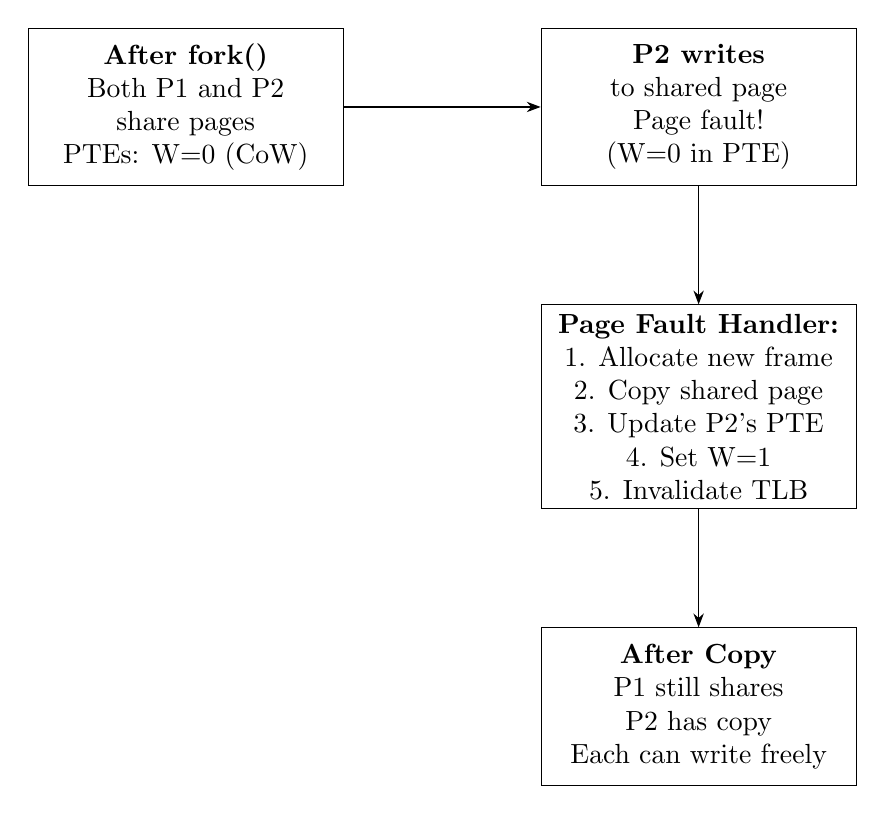
\begin{tikzpicture}[node distance=1.5cm, every text node part/.style={align=center}]

    % Initial state box
    \node[draw, rectangle, minimum width=4cm, minimum height=2cm] (init_state) {
        \textbf{After fork()} \\
        Both P1 and P2 \\
        share pages \\
        PTEs: W=0 (CoW)
    };

    % Arrow to write attempt
    \node[right=of init_state, xshift=1cm, draw, rectangle, minimum width=4cm, minimum height=2cm] (write_attempt) {
        \textbf{P2 writes} \\
        to shared page \\
        Page fault! \\
        (W=0 in PTE)
    };

    \draw[-{Stealth[length=5pt]}] (init_state) -- (write_attempt);

    % Arrow to page fault handler
    \node[below=of write_attempt, draw, rectangle, minimum width=4cm, minimum height=2.5cm] (handler) {
        \textbf{Page Fault Handler:} \\
        1. Allocate new frame \\
        2. Copy shared page \\
        3. Update P2's PTE \\
        4. Set W=1 \\
        5. Invalidate TLB
    };

    \draw[-{Stealth[length=5pt]}] (write_attempt) -- (handler);

    % Arrow to final state
    \node[below=of handler, draw, rectangle, minimum width=4cm, minimum height=2cm] (final_state) {
        \textbf{After Copy} \\
        P1 still shares \\
        P2 has copy \\
        Each can write freely
    };

    \draw[-{Stealth[length=5pt]}] (handler) -- (final_state);

\end{tikzpicture}
\caption{Copy-on-Write Fork: From shared read-only pages to independent copies on write.}
\label{fig:cow_fork_flow}
\end{figure}

% ============================================================
\section{TikZ Diagram: Permission State Transitions}
% ============================================================

\begin{figure}[h]
\centering
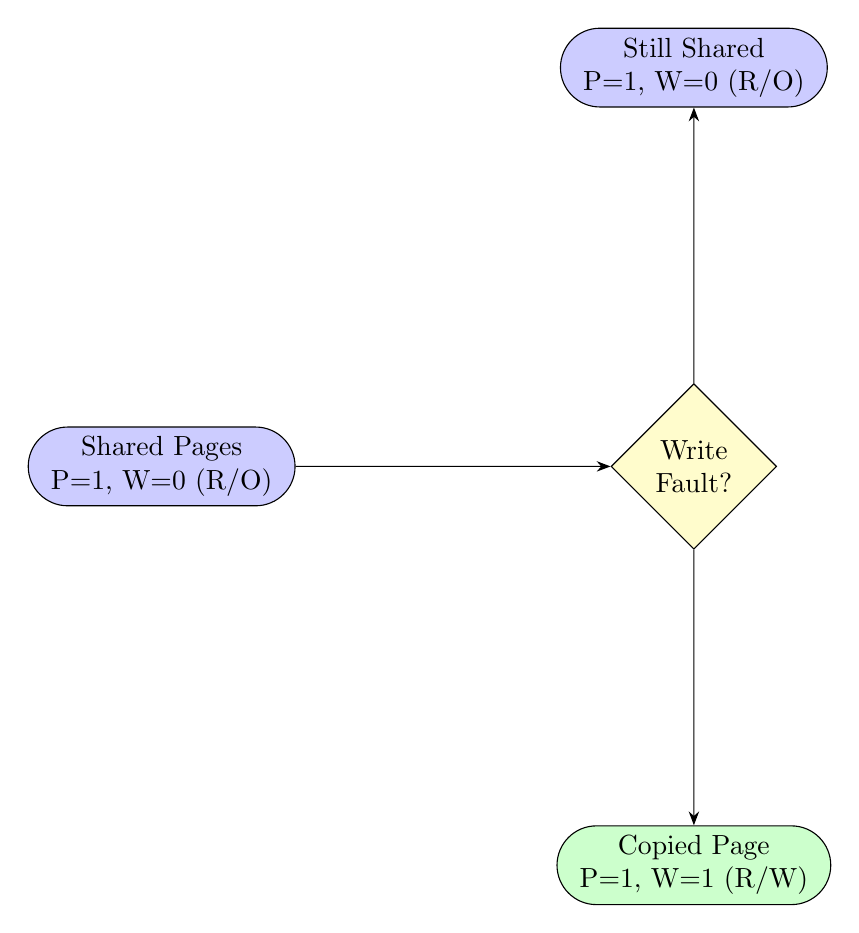
\begin{tikzpicture}[node distance=2cm]

    % Shared R/O state
    \node[draw, rounded rectangle, minimum width=3cm, minimum height=1cm, fill=blue!20, align=center] (shared_ro) {
        Shared Pages \\ P=1, W=0 (R/O)
    };

    % Write fault occurs
    \node[right=of shared_ro, xshift=2cm, draw, diamond, minimum width=2cm, minimum height=1.5cm, fill=yellow!20, align=center] (fault_event) {
        Write \\ Fault?
    };

    % Copy and restore
    \node[below=of fault_event, yshift=-1.5cm, draw, rounded rectangle, minimum width=3cm, minimum height=1cm, fill=green!20, align=center] (copied) {
        Copied Page \\ P=1, W=1 (R/W)
    };

    % No fault path
    \node[above=of fault_event, yshift=1.5cm, draw, rounded rectangle, minimum width=3cm, minimum height=1cm, fill=blue!20, align=center] (still_shared) {
        Still Shared \\ P=1, W=0 (R/O)
    };

    % Arrows
    \draw[-{Stealth[length=5pt]}] (shared_ro) -- (fault_event);
    \draw[-{Stealth[length=5pt]}, label={[right] Copy page}] (fault_event) -- (copied);
    \draw[-{Stealth[length=5pt]}, label={[left] No write}] (fault_event) -- (still_shared);

\end{tikzpicture}
\caption{Permission state transitions in copy-on-write: shared read-only pages become private read-write on write, or remain shared if never written.}
\label{fig:permission_transitions}
\end{figure}

% ============================================================
\section{Research Perspective: VM Cloning and Beyond}
% ============================================================

Copy-on-write fork is not merely a foundational OS technique; it has inspired decades of research into efficient memory sharing, VM cloning, and resource multiplexing. Several landmark research systems illustrate the power and limitations of CoW:

\textbf{Snowflock (EuroSys 2009, awarded Test of Time in EuroSys 2023)} provides rapid, on-demand VM cloning for cloud computing. It combines CoW page sharing with selective demand paging: only the pages that are accessed are transferred from the parent VM to the child clone. A fork of a 1-GB VM completes in milliseconds, and pages are transferred lazily over the network. This enables elastic scaling in the cloud, where spawning a new VM instance becomes as fast as spawning a process.

\textbf{Kaleidoscope (EuroSys 2011)} extends the idea to \emph{stateful VM replication}. By tracking which pages are read-only (can be safely shared) and which are modified by the VM workload, Kaleidoscope uses CoW to create efficient replicas for parallel execution, disaster recovery, and intrusion detection. Pages are selectively transferred and synchronized, enabling fine-grained control over VM state replication.

\textbf{On-Demand-Fork (EuroSys 2021)} revisits the fundamental question: can we do better than page-level CoW by extending CoW to page table pages (PTP CoW)? On-Demand-Fork shows that applying CoW at the page table level, not just the page level, yields dramatic speedups. For a 1-GB allocated address space, On-Demand-Fork achieves a \textbf{65x improvement} in fork latency compared to a naive fork without PTP CoW. In macro benchmarks, it achieves 59--226\% throughput improvement. Importantly, it reduces the number of fork invocations by 99\%, eliminating a primary source of overhead in many multi-process applications.

These research systems demonstrate that while page-level CoW is mature and widely deployed, the opportunity for further optimization remains. The core principles---lazy evaluation, interposition via page tables, and reference counting---are timeless. Modern systems continue to build upon these foundations.

% ============================================================
\section{Summary}
% ============================================================

\begin{itemize}
    \item \textbf{The lazy design principle:} Virtual memory's layer of indirection allows the OS to lie and defer action until necessary, enabling powerful optimizations.
    \item \textbf{Naive fork is wasteful:} Immediately duplicating all physical pages on \texttt{fork()} is expensive and often unnecessary.
    \item \textbf{Copy-on-write fork:} Both parent and child initially share the same physical pages, with all pages marked read-only. On a write, a page fault occurs, the OS copies the page, updates the child's PTE, and restores write permission.
    \item \textbf{Logical vs. physical permissions:} A page may be logically writable but physically read-only, allowing the OS to interpose on writes.
    \item \textbf{PTE flags and AVL bits:} The W (Writable) bit and P (Present) bit control page accessibility; AVL bits allow OS-specific metadata like CoW markers.
    \item \textbf{Reference counting:} Efficient CoW requires per-physical-page reference counts to track sharing and determine when a page can be made writable without future faults.
    \item \textbf{TLB management:} Page fault handlers must invalidate stale TLB entries; multiprocessor systems require TLB shootdown.
    \item \textbf{Engineering challenges:} Real implementations must handle nested forks, out-of-memory conditions, and cleanup of orphaned pages.
    \item \textbf{Aggressive deduplication:} Page table page CoW (PTP CoW) can further reduce fork overhead and memory usage, though it complicates the design.
    \item \textbf{Research directions:} Systems like Snowflock, Kaleidoscope, and On-Demand-Fork show that CoW principles extend to VM cloning, demand paging, and hybrid page/PTP CoW, enabling dramatic performance gains for cloud and multi-process workloads.
\end{itemize}

% ============================================================
\section{References}
% ============================================================

\begin{itemize}
    \item Intel Corporation. ``Intel 64 and IA-32 Architectures Software Developer's Manual.'' \textit{Volume 3: System Programming Guide}. 2023.
    \item Levy, Henry M., and Peter H. Lipman. ``Virtual Memory Management in the VAX.'' \textit{Computer Architecture News}, Vol. 10, No. 2, 1982.
    \item Waldspurger, Carl A. ``Memory Resource Management in VMware ESX Server.'' \textit{Proceedings of the USENIX Symposium on Operating Systems Design and Implementation (OSDI)}, 2002.
    \item Tanenbaum, Andrew S., and Herbert Bos. \textit{Modern Operating Systems}. 4th ed. Pearson, 2014.
    \item Barham, Paul, et al. ``Xen and the Art of Virtualization.'' \textit{Proceedings of the ACM Symposium on Operating Systems Principles (SOSP)}, 2003.
    \item Henson, Benjamin, et al. ``Snowflock: Rapid Virtual Machine Cloning for Cloud Computing.'' \textit{Proceedings of EuroSys}, 2009. \url{https://www.cs.cmu.edu/~dga/papers/snowflock-eurosys09.pdf}
    \item Koh, Youngjin, et al. ``Kaleidoscope: Cloud Resource Optimization at Microsecond Granularity.'' \textit{Proceedings of EuroSys}, 2011.
    \item Kwon, Min Soo, et al. ``On-Demand-Fork: A Better Fork() for Serverless Functions.'' \textit{Proceedings of EuroSys}, 2021.
    \item Silberschatz, Abraham, Peter B. Galvin, and Greg Gagne. \textit{Operating System Concepts}. 10th ed. Wiley, 2018.
    \item MIT Course 6.828: ``Operating System Engineering.'' \url{https://pdos.csail.mit.edu/6.828/}
    \item University of Washington CSE 451: ``Operating Systems.'' \url{https://courses.cs.washington.edu/courses/cse451/}
\end{itemize}

% ============================================================
\section*{Personal Notes}
% ============================================================
% Add your own notes below this line

\end{document}
